\section{Ejercicio 5}


\subsection{Desarrollo}
En el ejercicio se pide diseñar un lote con tres tareas de 50 ciclos y dos de 5 llamadas bloqueantes de 3 ciclos de duración. El lote que representamos inicia todas las tareas a la vez
\begin{verbatim}
TaskCPU 50
TaskCPU 50
TaskCPU 50
TaskConsola 5 3 3
TaskConsola 5 3 3
\end{verbatim}
Ejecutamos el lote con el scheduler \verb|SchedRR| para quantums 2, 10 y 50 como se pidió en el ejercicio. Utilizamos un solo cpu con cambio de contexto de 2 ciclos y  calculamos la latencia (tiempo desde que se carga la tarea hasta que comienza a ejecutarse), waiting time (tiempo en que la tarea permanece como READY) y el tiempo total de ejecución (tiempo desde que se cargó la tarea hasta que finalizó).  Para los cálculos utilizamos los siguientes tiempos (como ciclos) y su forma de obtenerlos del diagrama de Gantt:
\begin{description}
\item[ciclos] Cantidad de ciclos que permanece una tarea en estado RUNNING.\\
Para \verb|TaskCPU| de parámetro 50, el valor correspondiente es 51 (50 ciclos de uso de CPU más 1 ciclo para EXIT)\\
Para \verb|TaskConsola| de parámetros 5 3 3, son 21 ciclos, pues son 5 ciclos de E/S de 3 ciclos de duración más 1 ciclo de CPU cada E/S más un ciclo para EXIT (15 + 5 +1).
\item[inicio] Tiempo en el que se carga la tarea. Todas las tareas se cargan en el ciclo 0.
\item[fin] Tiempo en el que finaliza la tarea. En el diagrama de Gantt es en el ciclo en el que se realiza el UNLOAD.
\item[latencia] Cantidad de ciclos desde que se carga la tarea hasta que comienza a correr por primera vez.
\item[tiempo total] Tiempo que tarda la tarea en ejecutarse. En el diagrama de Gantt es la diferencia entre el ciclo en el que termina la tarea y el que se carga: fin - inicio.
\item[waiting time] Tiempo en el que la tarea permanece sin hacer nada: tiempo total - tiempo que corre la tarea
\end{description}
\subsection{Experimentación}
En las figuras \ref{fig:ej5q2},  \ref{fig:ej5q10} y \ref{fig:ej5q50} se representaron los diagramas de Gantt para los quantums 2, 10 y 50 respectivamente. Se puede ver, cómo a quantums más chicos (figura \ref{fig:ej5q2}), el scheduler permanece considerable tiempo haciendo cambios de contexto de 2 ciclos. Aún así, en quantums chicos, las tareas de E/S terminan antes que con los quantums más grandes.\par
\begin{figure}[H]
  \centering
    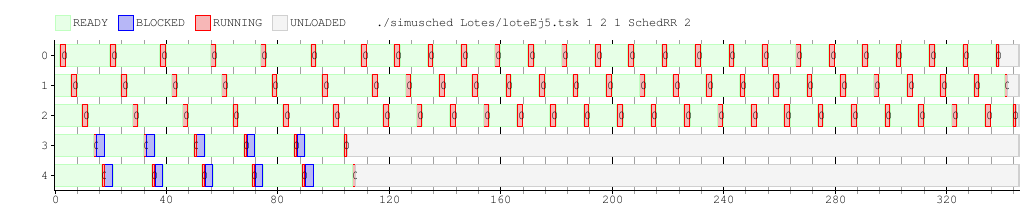
\includegraphics[width=1.1\textwidth]{imagenes/Ej5_q2.png}
  \caption{loteEj5.tsk con RR y quantum 2}\label{fig:ej5q2}
\end{figure}
Para quantums más grandes, todas las tareas terminan muy próximas entre sí, pero a quantums de 50 (figura \ref{fig:ej5q50}), las tareas de E/S comienzan luego de 150 ciclos (los tres quantums de las tareas de CPU) y podría parecer que el SO no responde.\par
\begin{figure}[H]
  \centering
    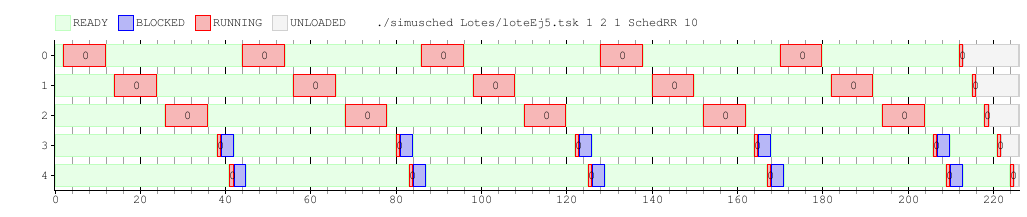
\includegraphics[width=1.1\textwidth]{imagenes/Ej5_q10.png}
  \caption{loteEj5.tsk con RR y quantum 10}\label{fig:ej5q10}
\end{figure}
\begin{figure}[H]
  \centering
    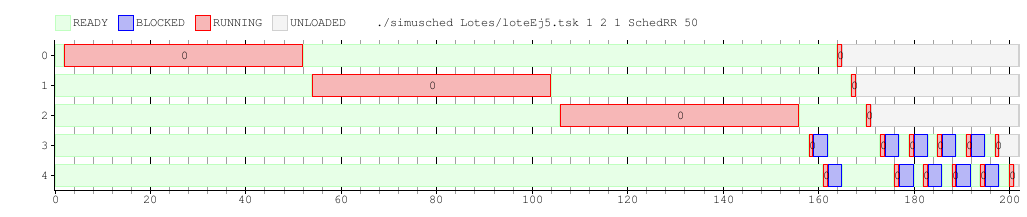
\includegraphics[width=1.1\textwidth]{imagenes/Ej5_q50.png}
  \caption{loteEj5.tsk con RR y quantum 50}\label{fig:ej5q50}
\end{figure}

En las tablas \ref{tab:ej5q2},  \ref{tab:ej5q10} y \ref{tab:ej5q50} se representaron los tiempos pedidos (como ciclos) para los quantums 2, 10 y 50 respectivamente.
\begin{table}[H]
\centering
\begin{tabular}{ | c | c | c | c | c | c | c | }
  \hline			
  pid & ciclos & inicio & fin & latencia & waiting time & tiempo total  \\
  \hline
 0 & 51 & 0 & 339 & 2 & 288 & 339\\
1 & 51 & 0 & 342 & 6 & 291 & 342\\
2 & 51 & 0 & 345 & 10 & 294 & 345\\
3 & 21 & 0 & 105 & 14 & 84 & 105\\
4 & 21 & 0 & 108 & 17 & 87 & 108\\
  \hline
promedio & - & - & - & 9.8 & CPU: 291  & CPU: 342 \\
                & &  &  &  & E/S: 85.5  & E/S: 106.5\\
  \hline
\end{tabular}
\caption{Tiempos para loteEj5.tsk con RR y quantum 2}\label{tab:ej5q2}
\end{table}

\begin{table}[H]
\centering
\begin{tabular}{ | c | c | c | c | c | c | c | }
  \hline			
  pid & ciclos & inicio & fin & latencia & waiting time & tiempo total  \\
  \hline
0 & 51 & 0 & 213 & 2 & 162 & 213\\
1 & 51 & 0 & 216 & 14 & 165 & 216\\
2 & 51 & 0 & 219 & 26 & 168 & 219\\
3 & 21 & 0 & 222 & 38 & 201 & 222\\
4 & 21 & 0 & 225 & 41 & 204 & 225\\
  \hline
promedio & - & - & - & 24.2 & CPU: 165  & CPU: 216\\
                & &  &  &  & E/S: 202.5  & E/S: 223.5\\
\hline
\end{tabular}
\caption{Tiempos para loteEj5.tsk con RR y quantum 10}\label{tab:ej5q10}
\end{table}

\begin{table}
\centering
\begin{tabular}{ | c | c | c | c | c | c | c | }
  \hline			
  pid & ciclos & inicio & fin & latencia & waiting time & tiempo total  \\
  \hline
0 & 51 & 0 & 165 & 2 & 114 & 165\\
1 & 51 & 0 & 168 & 54 & 117 & 168\\
2 & 51 & 0 & 171 & 106 & 120 & 171\\
3 & 21 & 0 & 198 & 158 & 177 & 198\\
4 & 21 & 0 & 201 & 161 & 180 & 201\\
  \hline
promedio & - & - & - & 96.2 & CPU: 117  & CPU: 168 \\
                & &  &  &  & E/S: 178.5  & E/S: 199.5\\
  \hline
\end{tabular}
\caption{Tiempos para loteEj5.tsk con RR y quantum 50}\label{tab:ej5q50}
\end{table}
Lo que podemos notar de las tablas, es que con quantums chicos, la latencia es menor, pero cuando hay muchas tareas de uso intenso de CPU, éstas tardan más en terminar debido a los constantes cambios de contexto. Para quantums más grandes, los proceso E/S parecen sufrir de inaninción, pues se ejecutan primero los proceso de CPU que son largos.\par